\chapter{Support Vector Machines}

Support Vector Machine are a set of related supervised learning methods used for classification and regression. They belong to a family of generalized linear classifiers. In other terms, SVM is a classification and regression prediction tool that uses machine learning theory to maximize predictive accuracy while automatically avoiding overfit to the data. They became famous when, using pixel maps as input, they give accuracy comparable to sophisticated neural networks with elaborated features in a handwriting recognition task. It is also being used for many applications, such as hand writing analysis, face analysis and so fort, especially for pattern classification and regression based applications.

\begin{wrapfigure}{r}{0.35\textwidth}
    \begin{center}
        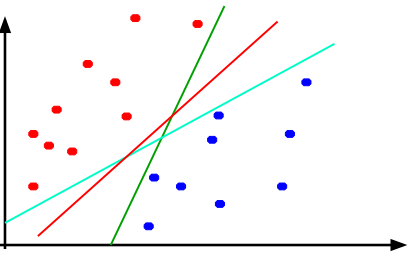
\includegraphics[width=0.35\textwidth]{041}
        \caption{Possible hyperplanes for linearly-separable data that shows the best solution (red middle line) compared to other possible solutions.}
        \label{fig:041}
        \vspace*{-10pt}
    \end{center}
\end{wrapfigure}

Let's start by thinking back to the original goal of linear classifiers: to find a hyperplane that separates the positive training examples from the negative ones. Figure~\ref{fig:041} shows some data and three potential hyperplane that separates the red training examples from the blue one. Which one do you like the best? Most likely you chose the red hyperplane. And most likely you chose it because it was furthest away from the closest training points. In other words, it has a large \textbf{margin}. The desire for hyperplanes with large margins is a perfect example of an inductive bias\footnote{\textbf{Inductive Bias} play an important role in the ability of models to generalize to the unseen data. A strong inductive bias can lead our model to converge to the global optimum, on the other hand, a weak inductive bias can cause the model to find only the local optima and be greatly affected by random changes in the initial states.}. Following this line of thinking leads us to the \textbf{Support Vector Machine} (SVM). this is simply a way of setting up an optimization problem that attempts to find a separating hyperplane with as large margin as possible. 

\section{Large margin classifiers}
The \textbf{margin} of a single data point is defined to be the distance from the data point to a decision boundary. Note that there are many distances and decision boundaries that may be appropriate for certain datasets and goals.

A \textbf{margin classifier} is a classifier which is able to give an associated distance from the decision boundary for each example. For instance, if a linear classifier is used, the distance of an example from the separating hyperplane is the margin of that example.

There are many hyperplanes that might classify the data. One reasonable choice of the best hyperplane is the one that represents the largest margin between the two classes. So we choose the hyperplane so that the distance from it to the nearest data point on each side is maximized. If such a hyperplane exists, it is known as the \textbf{maximum margin hyperplane} and the linear classifier it defines is known as a \textbf{maximum margin classifier}, or equivalently, the perceptron of optimal stability.
\begin{wrapfigure}{l}{0.4\textwidth}
    \begin{center}
        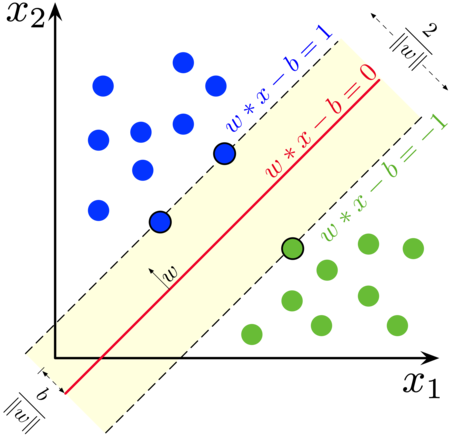
\includegraphics[width=0.35\textwidth]{042}
        \caption{Maximum-margin hyperplane and margins for an SVM trained with samples from two classes.}
        \label{fig:042}
    \end{center}
    \vspace*{-40pt}
\end{wrapfigure}
\subsection{Support vectors}
Support vectors are the elements of the training set that would change the position of the dividing hyperplane if removed. They are critical elements of the training set. Support vectors are observations that lie on the margin surrounding the data-separating hyperplane. Since the margin defines the minimum distance observations should have from the plane, the observations that lie on the margin impact the orientation and position of the hyperplane.

The problem of finding the optimal hyperplane is an optimization problem and can be solved by optimization techniques. For \(n\) dimensions, there will be at least \(n+1\) support vectors. We can see in Figure~\ref{fig:042} that there are 3 support vectors, 2 are of the blue class, and 1 of the green class.

\subsection{Maximizing the margin}
Given the hyperplane in Figure~\ref{fig:042}, we have the margins described by the equation \(\vec{w} \cdot \vec{x} - b = a\), where \(a=1\) for the blue margin, and \(a=-1\) for the green margin. The measure for the margin is defined by
\begin{equation}
    \frac {\vec{w} \cdot \vec{x}_i + b} {||\vec{w}||} = \frac 1 {||\vec{w}||}
\end{equation}

Our goal is now to maximize the margin, namely, to select the hyperplane with the largest margin where the points are classified correctly and outside the margin. Let's setup the problem as a constrained optimization problem, subject to \(y_i(\vec{w} \cdot \vec{x}_i + b) \geq 1 \quad \forall i\)
\begin{align}
    \max_{a,b} margin(\vec{w},b) &= \max_{w,b} \frac 1 {||\vec{w}||}\\
    &= \min_{w,b} ||\vec{w}||
\end{align}
Maximizing the margin is equivalent to minimize the norm of the weights (subject to separating constraints). The minimization criterion wants \(\vec{w}\) to be as small as possible, while the constraints make sure that the data is separable.

The \textbf{support vector machine problem} is a version of a \textbf{quadratic optimization problem}, which wants to minimize a quadratic function subject to a set of linear constraints.
\begin{align*}
    &\min_{\vec{w},b} ||\vec{w}||^2\\
    \text{subject to: } &y_i(\vec{w} \cdot \vec{x}_i + b) \geq 1 \quad \forall i
\end{align*}

\section{Soft margin classification}
For the very high dimensional problems common in classification, sometimes the data are linearly separable. But in general case they are not, and even if they are, we might prefer a solution that better separates the bulk of the data while ignoring a few weird noise. 

If the training set \(D\) is not linearly separable, the standard approach is to allow the fat decision margin to make a few mistakes (some points - outliers or noisy example - are inside or on the wrong side of the margin). We then pay a cost for each misclassified example, which depends on how far it is from meeting the margin requirements. To implement this, we introduce \emph{slack variables} \(\zeta_i\). A non-zero value for \(\zeta_i\) allows \(\vec{x}_i\) to not meet the margin requirement at a cost proportional to the value of \(\zeta_i\).

The formulation of the SVM optimization problem with slack variables is: Find \(\vec{w}\), \(b\) and \(\zeta_i \geq 0\) such that:
\begin{itemize}
    \item
    \(\frac 1 2 \vec{w}^T \vec{w} + C \sum_i \zeta_i\) is minimized
    \item
    and \(\forall \{(\vec{x}_i, y_i)\}\), \(y_i(\vec{w}^T \vec{x}_i + b) \geq 1 - \zeta_i\)
\end{itemize}
\begin{align*}
    &\min_{\vec{w},b} ||\vec{w}||^2\\ + C \sum_i \zeta_i\\
    \text{subject to: } &y_i(\vec{w} \cdot \vec{x}_i + b) \geq 1 - \zeta_i \quad \forall i,\ \zeta \geq 0
\end{align*}

The optimization problem is then a trading off how fat it can make the margin versus how many points have to be moved around to allow this margin. the margin can be less than 1 for a point \(\vec{x}_i\) by setting \(\zeta_i > 0\), but then one pays a penalty of \(C\zeta_i\) in the minimization for having done that. The sum of the \(\zeta_i\) gives an upper bound on the number of training errors.

\begin{figure}[h!]
    \centering
    \begin{subfigure}{.4\textwidth}
        \centering
        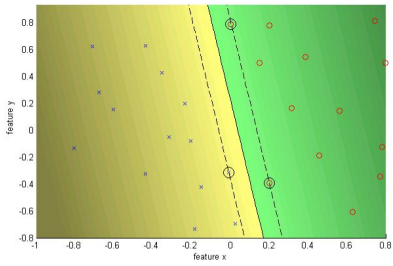
\includegraphics[width=1\textwidth]{043}
        \caption{\(C = \infty\) hard margin}
    \end{subfigure}
    \begin{subfigure}{.4\textwidth}
        \centering
        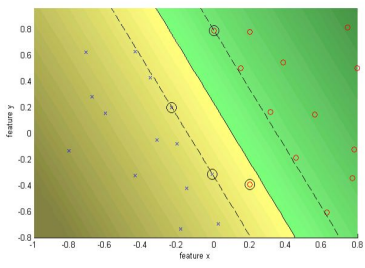
\includegraphics[width=1\textwidth]{044}
        \caption{\(C=10\) soft margin}
    \end{subfigure}
    \caption{Hard margin vs soft margin example.}
\end{figure}

Soft-margin SVMs minimize training error traded off against margin. The parameter \(C\) is a \emph{regularization term}, which proivdes a way to control overfitting: small \(C\) allows constraints to be easily ignored (large margin); large \(C\) makes constraints hard to ignore (narrow margin). If \(C = \infty\) enforces all constraints: \textbf{hard margin}. The slack variable can have two different values:
\begin{align}
    \zeta_i &= \begin{cases}
        0 &\text{if } y_i(\vec{w} \cdot \vec{x}_i + b) \geq 1\\
        1-y_i(\vec{w} \cdot \vec{x}_i + b) &\text{otherwise}\\
    \end{cases}\\
    &=\max(0, 1-y_i(\vec{w} \cdot \vec{x}_i + b))\\
    &=\max(0,1-yy')
\end{align}
Note that the last equality is the \textbf{hinge loss}, that is actually our loss, so we can rewrite our optimization problem as follows
\begin{equation}
    \min_{\vec{w},b} ||\vec{w}||^2 + C \sum_i \max(0,1-y_i(\vec{w} \cdot \vec{x}_i + b))
\end{equation}
That looks like the expression:
\begin{equation}
    arg \min_{\vec{w},b} \sum_i^n l(yy') + \lambda R(\vec{w} b)
\end{equation}

\section{Non linearly separable data}
We have gone though the understanding of \textbf{Support Vectors} and \textbf{Margins}. Then used the concepts to build the objective functions for soft margin classifier. We have have also learned the objective function, that is defined as \textbf{Primal Problem}. However our final goal is to solve non-linear SVM, where primal problem is not helpful, we need a procedure that increases the number of features in order to make our data linearly separable.

\subsubsection{Classes of Optimization Problems}
Let's revise some classes of optimization problems, in order to see where does the support vector machine objective function locate.

% paragraph  (end)
\paragraph{Linear Programming (LP)}
We have a linear problem, with linear constraints.
\begin{align*}
    &\min_{\vec{x}} \vec{c}^T \vec{x}\\
    \text{s.t. } &\vec{A} \vec{x} = b, \quad \vec{x} \geq 0
\end{align*}

\paragraph{Quadratic Programming (QP)}
We have a quadrative objective and linear constraints. It is convex if \(Q\) is positive semidefinite.
\begin{align*}
    &\min_{\vec{x}} \vec{c}^T \vec{x} + \frac 1 2 \vec{X}^T Q \vec{x}\\
    \text{s.t. } &\vec{A}\vec{x} = b, \quad C\vec{x} \geq d
\end{align*}

\paragraph{Nonlinear Programming (NLP)}
In general it is not convex.
\begin{align*}
    &\min_{\vec{x}} f(\vec{x})\\
    \text{s.t. } &g(\vec{x}) = 0, \quad h(\vec{x}) \geq 0
\end{align*}

\subsection{Dual problem}
In mathematical optimization theory, duality means that optimization problems may be viewed from either of two perspectives, the primal problem or the dual problem. The solution to the dual problem provides a lower bound to the solution of the primal (minimization) problem.

Quadratic optimization problems are a well-known class of mathematical programming problems for which several algorithms exist. One possible solution involves constructing a dual problem where a Lagrange multiplier \(\alpha_i\) is associated with every inequality constraint in the primal problem:

Find \(\alpha_1, ..., \alpha_n\) such that \(\sum_i \alpha_i - \frac 1 2 \sum_i \sum_j \alpha_i \alpha_j y_i y_j \vec{x}_i^T \vec{x}_j\) is maximized and
\begin{itemize}
    \item
    \(\sum_i \alpha_i y_i = 0\)\\
    \item
    \(\alpha_i \geq 0,\ \forall i\)
\end{itemize}

Given a solution \(\alpha_1...\alpha_n\) to the dual problem, the solution to the primal is:
\begin{align*}
    \vec{w} &= \sum_i \alpha_i y_i \vec{x}_i\\
    b &= y_k - \sum_i \alpha_i y_i \vec{x}_i^T \vec{x}_k \text{ for any } \alpha_k > 0
\end{align*}
Each non-zero \(\alpha_i\) indicates that the corresponding \(\vec{x}_i\) is a support vector. Then the classifying function is:
\begin{equation}
    f(\vec{x}) = \sum_i \alpha_i y_i \vec{x}_i^T \vec{x} + b
\end{equation}
The solution relies on an inner product between the test point \(\vec{x}\) and the support vectors \(\vec{x}_i\). Also solving the optimization problem involves the computing of the inner products between all training points.

Dual problem is similar in the non separable case, but notice the constraints.

Find \(\alpha_1...\alpha_N\) such that \(\sum_i \alpha_i - \frac 1 2 \sum_i \sum_j \alpha_i \alpha_j y_i y_j \vec{x}_i^T \vec{x}_j\) is maximized and
\begin{itemize}
    \item \(\sum_i \alpha_i y_i = 0\)\\
    \item \(0 \geq \alpha_i \geq C\) for all \(\alpha_i\)
\end{itemize}
Again, \(\vec{x}_i\) with non-zero \(\alpha_i\) represent support vectors.

\subsection{Kernel trick}
Suppose now that we would like to learn a nonlinear classification rule which corresponds to a linear classification rule for the transformed data points \(\phi(\vec{x}_i)\). The linear classifier relies on inner product between vectors
\begin{equation}
    K(\vec{x}_i,\vec{y}_j) = \vec{x}_i^T \vec{x}_j
\end{equation}
\begin{figure}[h]
    \centering
    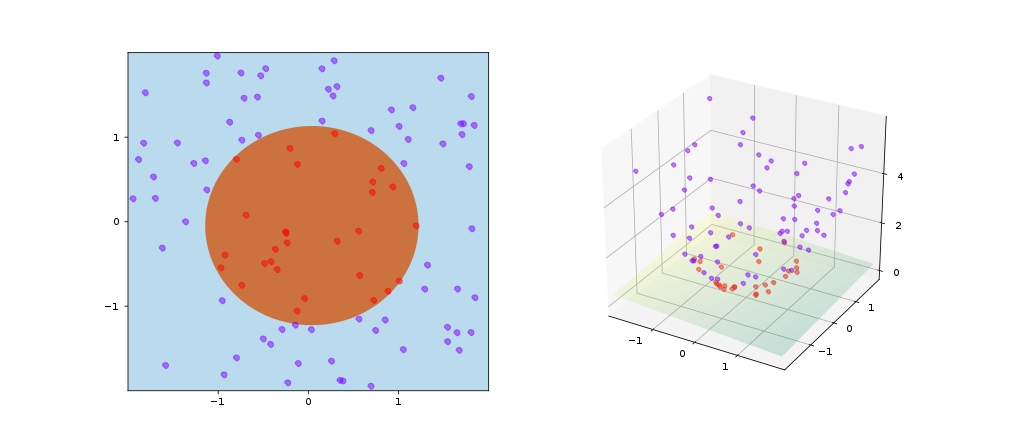
\includegraphics[width=1\textwidth]{045}
    \caption{A training example of SVM with kernel given by \(\phi((a,b)) = (a,b,a^2+b^2)\)}
\end{figure}
If every datapoint is mapped into high-dimensional space via some transformation \(\Phi: \vec{x} \to \phi(\vec{x})\), the inner product becomes
\begin{equation}
    K(\vec{x}_i,\vec{x}_j) = \phi(\vec{x}_i)^T \phi(\vec{x}_j)
\end{equation}
A kernel function is a function that is equivalent to an inner product in some feature space. It \textbf{implicitly} maps data to a high-dimensional space (without the need to compute each \(\phi(\vec{x})\) explicitly).

For some function \(K(\vec{x}_i,\vec{x}_j)\) checking that \(K(\vec{x}_i,\vec{x}_j) = \phi(\vec{x}_i)^T \phi(\vec{x}_j)\) can be cumbersome.

\subsubsection{Mercer's theorem}
Every positive semidefinite symmetric\footnote{A symmetric matrix is \textbf{positive semidefinite} if and only if all eigenales are non-negative} function is a kernel. A positive semidefinite symmetric function correspond to a positive semidefinite symmetric Gram matrix

\begin{equation}
    K = 
    \begin{bmatrix}
        K(\vec{x}_1,\vec{x}_1) & K(\vec{x}_1,\vec{x}_2) & ... & K(\vec{x}_1,\vec{x}_n) \\
        K(\vec{x}_2,\vec{x}_1) & K(\vec{x}_2,\vec{x}_2) & ... & K(\vec{x}_2,\vec{x}_n) \\
        ... & ... & ... & ... \\
        K(\vec{x}_n,\vec{x}_1) & K(\vec{x}_n,\vec{x}_2) & ... & K(\vec{x}_n,\vec{x}_n) 
    \end{bmatrix}
\end{equation}

\subsubsection{Kernels}
\begin{itemize}[topsep=0pt, partopsep=0pt]
    \item Linear: \(K(\vec{x}_i,\vec{x}_j) = \vec{x}_i^T\vec{x}_j\)\\
    \item Polynomial of power \(p\): \(K(\vec{x}_i,\vec{x}_j) = (1 + \vec{x}_i^T \vec{x}_j)^p\)\\
    \item Gaussian (radial-basis function): \(K(\vec{x}_i,\vec{x}_j) = e^{\frac {||\vec{x}_i - \vec{x}_j||^2} {2 \sigma^2}}\)\\
        \begin{itemize}
        \item Mapping \(\Phi: \vec{x} \to \phi(\vec{x})\), where \(\phi(\vec{x})\) is infinite-dimensional: every point is mapped to a function (Gaussian); combination of functions for support vectors is the separator.\\
        \end{itemize}
\end{itemize}
Higher-dimensional space still has \emph{intrinsic} dimensionality \(d\) (the mapping is \emph{onto}), but linear separators in it correspond to non-linear separators in original space.

With the kernels, the dual problem formulation becomes
\begin{align*}
    &\max_\alpha \sum_i \alpha_i - \frac 1 2 \sum_i \sum_j \alpha_i \alpha_j y_i y_j K(\vec{x}_i, \vec{x}_j)\\
    \text{s.t. } &\sum_i \sum_j \alpha_i y_i = 0, \quad \alpha_i \geq 0, \quad \forall i
\end{align*}
And finally the solution is
\begin{equation}
    f(\vec{x}) = \sum_i \alpha_i y_i K(\vec{x}_i; \vec{x}) + b
\end{equation}
The optimization techniques for finding \(\alpha_i\)'s remains the same.

\newpage
\begin{exercise}[topsep=20pt, itemsep=10pt]
    \ex[!] Describe the Support Vector Machine.
    \ex What are large margin classifiers?
    \ex What is a support vector?
    \ex How do we maximize the margin?
    \ex[!] What is the Support Vector Machine Problem?
    \ex Describe the soft margin classification.
    \ex What are the slack variables? What are they used for?
    \ex[!] Why do we need the slack variables?
    \ex What if we have non linearly separable data?
    \ex Why do we need the dual problem?
    \ex Describe the kernel trick for Support Vector Machine.
    \ex Explain the Mercer's theorem.
    \ex What is a kernel?
    \ex How does the dual problem formulation become with kernels?
    \ex[!] Does SVM use regularization? What regularizer does SVM use?
    \ex[!] Compare SVM with \(k\)-NN.
\end{exercise}
